\section{Abstract Classes}

We consider a class to be abstract if it is not representable by any instance. That is, we cannot create an instance of an abstract class. Abstract classes are useful when we want to define a class that is a generalization of other classes, but we do not want to create instances of the generalization.

\myexample{Consider, once again, a hierarchy of animals.} There is no such thing as an ``animal'' or something that is solely called an animal. On the other hand, everything that we would categorize as an animal \emph{is} an animal. Therefore it makes sense to say that animals are a generalization of other types of ``sub''-animals. Imagine we want to write an \ttt{Animal} class, where we will say that any animal can speak. The abstract class contains a superfluous constructor as well as an abstract \ttt{speak} method. We define \ttt{speak} as abstract to denote that an animal can speak, but it is nonsensical for \ttt{Animal} to speak. Because it is impossible to instantiate an instance of \ttt{Animal}, it is similarly impossible to reasonably define \ttt{speak}.

\enlargethispage{-2\baselineskip}
\begin{lstlisting}[language=MyJava]
abstract class Animal {

  Animal() {} 

  abstract String speak();
}
\end{lstlisting}

Let's declare two subclasses: \ttt{Dog} and \ttt{Cat}, representing dogs and cats respectively. A cat can meow via the string \ttt{"Meow!"}, whereas a dog woofs via the string \ttt{"Woof!"}. 

\begin{lstlisting}[language=MyJava]
class Dog extends Animal {

  Dog() { super(); }

  @Override
  String speak() { return "Woof!"; }
}
\end{lstlisting}

\begin{lstlisting}[language=MyJava]
class Cat extends Animal {

  Cat() { super(); }

  @Override
  String speak() { return "Meow!"; }
}
\end{lstlisting}

It might seem strange to use an abstract class, since we could write a \ttt{Speakable} interface to do the same logic. The differences between abstract classes and interfaces is a blurry line to beginning Java programmers (and even to some who have been programming for years), but in essence, we use abstract classes when we want to enforce a class hierarchy of ``is-a'' relationships, e.g., a \ttt{Cat} is-a \ttt{Animal}, and a \ttt{Dog} is-a \ttt{Animal}. Moreover, abstract classes can contain non-abstract methods, meaning that a subclass needs not to override such methods. Interfaces, on the other hand, contain only methods that the implementing class must override. In addition to the method distinction, abstract classes may contain instance variables, whereas interfaces may not.\footnote{Both abstract classes and interfaces can contain static methods and variables.}

\myexample{Suppose we're writing a two-dimensional game that has different types of interactable objects in the world. The core game object stores the $(x, y)$ location, with nothing more. Again, we want to design a class that specific types of game objects can extend. For instance, our game might contain circular and rectangular objects. Of course, circles and rectangles have different dimension units, namely radius versus width and height respectively. We plan for each object to be interactable with one another. Unfortunately, collision detection is a complicated set of algorithms whose discussion far exceeds the scope of this text. Conversely, there is an extremely straightforward solution that involves treating all objects as rectangles. We call this technique \emph{axis-aligned bounding box}. Because not every object may be collidable, we will design a class \ttt{AxisAlignedBoundingBoxObject} that separately stores the object width and height as the dimensions of the bounding box. This class defines a method for colliding with another \ttt{AxisAlignedBoundingBoxObject}, which determines whether some point of $o_1$ is inside the bounding box of the $o_2$ object. This logic is not the focal point of the discussion, so we will only illustrate the example via an image and not explain the code itself. The purpose for this example is to demonstrate object hierarchy; not recreate the next best-selling two-dimensional side-scroller.}

\begin{figure}[H]
\centering
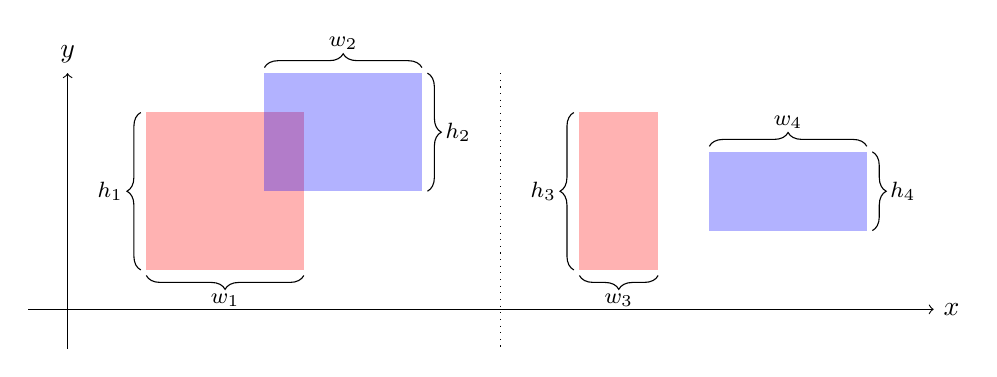
\begin{tikzpicture}[scale=1]

% Coordinates of Rectangle 1
\coordinate (A) at (1, .5);
\coordinate (B) at (3, .5);
\coordinate (C) at (3, 2.5);
\coordinate (D) at (1, 2.5);

% Coordinates of Rectangle 2
\coordinate (E) at (2.5, 1.5);
\coordinate (F) at (4.5, 1.5);
\coordinate (G) at (4.5, 3);
\coordinate (H) at (2.5, 3);

% Draw x/y axis
\draw[->] (-.5,0) -- (11,0) node[right] {\textbf{$x$}};
\draw[->] (0,-.5) -- (0,3) node[above] {\textbf{$y$}};
\draw[dotted] (5.5, 3) -- (5.5,-.5) node[above] {};

% Draw Rectangle 1 in transparent red
\fill[red, opacity=0.3] (A) -- (B) -- (C) -- (D) -- cycle;

% Draw Rectangle 2 in transparent blue
\fill[blue, opacity=0.3] (E) -- (F) -- (G) -- (H) -- cycle;

% Width labels for Rectangle 1
\draw[decorate, decoration={brace, amplitude=5pt, mirror, raise=2pt}] (A) -- (B) node[midway, below=5pt] {\footnotesize{}$w_1$};
\draw[decorate, decoration={brace, amplitude=5pt, raise=2pt}] (A) -- (D) node[midway, left=5pt] {\footnotesize{}$h_1$};

% Width labels for Rectangle 2
\draw[decorate, decoration={brace, amplitude=5pt, raise=2pt, mirror}] (G) -- (H) node[midway, above=5pt] {\footnotesize{}$w_2$};
\draw[decorate, decoration={brace, amplitude=5pt, raise=2pt, mirror}] (F) -- (G) node[midway, right=5pt] {\footnotesize{}$h_2$};

% Coordinates of Rectangle 3
\coordinate (I) at (6.5, .5);
\coordinate (J) at (7.5, .5);
\coordinate (K) at (7.5, 2.5);
\coordinate (L) at (6.5, 2.5);

% Coordinates of Rectangle 4
\coordinate (M) at (8.15, 1);
\coordinate (N) at (10.15, 1);
\coordinate (O) at (10.15, 2);
\coordinate (P) at (8.15, 2);

% Draw Rectangle 3 in transparent red
\fill[red, opacity=0.3] (I) -- (J) -- (K) -- (L) -- cycle;

% Draw Rectangle 4 in transparent blue
\fill[blue, opacity=0.3] (M) -- (N) -- (O) -- (P) -- cycle;

% Width labels for Rectangle 3
\draw[decorate, decoration={brace, amplitude=5pt, mirror, raise=2pt}] (I) -- (J) node[midway, below=5pt] {\footnotesize{}$w_3$};
\draw[decorate, decoration={brace, amplitude=5pt, raise=2pt}] (I) -- (L) node[midway, left=5pt] {\footnotesize{}$h_3$};

% Width labels for Rectangle 4
\draw[decorate, decoration={brace, amplitude=5pt, raise=2pt, mirror}] (O) -- (P) node[midway, above=5pt] {\footnotesize{}$w_4$};
\draw[decorate, decoration={brace, amplitude=5pt, raise=2pt, mirror}] (N) -- (O) node[midway, right=5pt] {\footnotesize{}$h_4$};
\end{tikzpicture}
\caption{Collision Detection Between Rectangles.}
\label{fig:collisiondetection}
\end{figure}

%\enlargethispage{1\baselineskip}
\begin{lstlisting}[language=MyJava]
abstract class GameObject {
  
  private int x;
  private int y;

  GameObject(int x, int y) {
    this.x = x;
    this.y = y;
  }
}
\end{lstlisting}


\begin{lstlisting}[language=MyJava]
abstract class AxisAlignedBoundingBoxObject extends GameObject {
  
  private int width;
  private int height;

  AxisAlignedBoundingBoxObject(int x, int y, int width, int height) {
    super(x, y);
    this.width = width;
    this.height = height;
  }

  /**
   * Determines whether this object collides with 
   * another AxisAlignedBoundingBoxObject.
   * @param obj instance of AxisAlignedBoundingBoxObject.
   * @return true if the objects overlap and false otherwise.
   */
  boolean collidesWith(AxisAlignedBoundingBoxObject obj) {
    return (this.getX() < obj.getX() + obj.width) &&
	   (this.getX() + this.width >= obj.getX()) &&
 	   (this.getY() < obj.getY() + obj.height)  &&
	   (this.getY() + this.height >= obj.height); 
  }
}
\end{lstlisting}

We declared an abstract class to extend another abstract class; which is perfectly acceptable. Because it makes no sense to instantiate an entity, in and of itself, called \ttt{AxisAlignedBoundingBoxObject}, we declare it as abstract, but we need it to contain the functionality of \ttt{GameObject}, which calls for the inheritance. Normally, we would immediately write an extensive test suite for \ttt{collidesWith}, but because we cannot instantiate an \ttt{AxisAlignedBoundingBox} directly, we cannot test \ttt{collidesWith} at the moment. In a couple of paragraphs, however, this will be possible, with the additions of \ttt{CircleObject} and \ttt{RectangleObject}.

%\enlargethispage{4\baselineskip}
\begin{lstlisting}[language=MyJava]
import static Assertions.assertAll;
import static Assertions.assertEquals;

class AxisAlignedBoundingBoxObjectTester {

  @Test
  void testCollidesWith() {
    AxisAlignedBoundingBoxObject o1 
      = new RectangleObject(30, 30, 1000, 2000);
    AxisAlignedBoundingBoxObject o2 
      = new RectangleObject(0, 0, 5, 5);
    AxisAlignedBoundingBoxObject o3 
      = new RectangleObject(400, 200, 750, 250);
    AxisAlignedBoundingBoxObject o4 
      = new RectangleObject(300, 100, 300, 200);
    AxisAlignedBoundingBoxObject o5 
      = new CircleObject(20, 30, 1000);
    AxisAlignedBoundingBoxObject o6 
      = new CircleObject(200, 250, 500);
    AxisAlignedBoundingBoxObject o7 
      = new CircleObject(30, 300, 1500);
    AxisAlignedBoundingBoxObject o8 
      = new CircleObject(90, 85, 200);
    assertAll(
      () -> assertTrue(o1.collidesWith(o2)),
      () -> assertTrue(o1.collidesWith(o4)),
      () -> assertTrue(o2.collidesWith(o3)),
      () -> assertTrue(o2.collidesWith(o8)),
      () -> assertTrue(o3.collidesWith(o5)),
      () -> assertTrue(o5.collidesWith(o4)),
      () -> assertTrue(o6.collidesWith(o7)),
      () -> assertTrue(o7.collidesWith(o3)));
  }
}
\end{lstlisting}

We need to translate our circles into axis-aligned bounding box, but what does that mean? In short, we convert the given radius into the corresponding diameter, and designate this diameter as the width and height of the bounding box. Rectangular objects, on other hand, need no such fancy translation, since a bounding box is a rectangle. Neither subclasses store their dimensions as instance variables, due to the fact that the superclass takes care of this for us.

The question that we anticipate many readers are thinking of is, why do we even distinguish objects of differing ``types'' if they both implement collision detection in the same fashion? Since we are working in the context of a game, the way we draw these objects is certainly different! Let's, for the sake of emphasizing the distinctions, design a \ttt{IDrawable} interface, which provides one method: \ttt{void draw(Graphics2D g2d)}, which gives us a \ttt{Graphics2D} object. We will not discuss, nor do we really care about the innards of a graphics library aside from the fact that it contains two primitive methods: \ttt{drawOval(int x, int y, int w, int h)} and \ttt{drawRect(int x, int y, int w, int h)}. Therefore our two object subclasses will implement \ttt{IDrawable} and override the method differently.

\enlargethispage{-4\baselineskip}
\begin{lstlisting}[language=MyJava]
interface IDrawable {
  
  /**
   * Provides a means of drawing primitive graphics.
   * The inner details of "Graphics2D" are not important to us; 
   * we care about the fact that we can use the following methods:
   * 
   * - drawOval(int x, int y, int w, int h);
   * - drawRect(int x, int y, int w, int h);
   */
  void draw(Graphics2D g2d); 
}
\end{lstlisting} 

%\enlargethispage{2\baselineskip}
\begin{lstlisting}[language=MyJava]
class CircleObject extends AxisAlignedBoundingBoxObject implements IDrawable {
  
  CircleObject(int x, int y, int r) { super(x, y, r * 2, r * 2); }

  @Override
  public void draw(Graphics2D g2d) {
    g2d.drawOval(this.getX(), this.getY(), 
                 this.getWidth(), this.getHeight());
  }
}
\end{lstlisting}

\begin{lstlisting}[language=MyJava]
class RectangleObject extends AxisAlignedBoundingBoxObject implements IDrawable {
  
  RectangleObject(int x, int y, int w, int h) { super(x, y, w, h); }
  
  @Override
  public void draw(Graphics2D g2d) {
    g2d.drawRect(this.getX(), this.getY(), 
                 this.getWidth(), this.getHeight());
  }
}
\end{lstlisting}

\myexample{A terminal argument parser is a program/function that interprets a series of arguments passed to another program and makes it easier for programmers to determine if a flag is enabled. Without one, many programmers often resort to using a complex series of conditional statements to check for the existence of a flag. Not only is this cumbersome, but it is prone to errors, and neither extendable nor flexible to different arrangements of arguments. In this example we will develop a small terminal argument parser.}

First, we need to design a class that represents an ``argument'' to a program. Arguments, as we described in Chapter~\ref{chapter-arrays-collections}, are space-separated string values that we pass to a program executable, which populate the \ttt{String[] args} array in the \ttt{main} method. In particular, however, we want to specify that an argument is not necessarily the values themselves, but are instead the flags, or instructions, passed to the executable. The simplest version of a flag is one that receives exactly one argument, which we will represent via an abstract \ttt{Argument} class. Later on, we want to be able to validate a flag with its given arguments, so the \ttt{Argument} class includes an abstract \ttt{boolean validate} method, that shall be overridden in all subclasses of \ttt{Argument}.

\begin{lstlisting}[language=MyJava]
import java.util.List;
import java.util.Map;

abstract class Argument {

  private String key;

  Argument(String key) { this.key = key; }

  String getKey() { return this.key; }

  abstract boolean validate(Map<String, List<String>> args);
}
\end{lstlisting}

From here, let's design two types of arguments: one that is optional and one that receives~$n$ arguments. Namely, an optional argument is one that is always valid, according to \ttt{validate}, because it does not necessarily need to exist. The~$n$-valued argument, on the other hand, requires that the associated passed flag contains exactly~$n$ values. For example, if we say that the \ttt{--input} flag requires exactly~$3$ arguments, then if we do not pass exactly three space-separated non-flag values, it fails to validate.

\begin{lstlisting}[language=MyJava]
import java.util.List;
import java.util.Map;

class OptionalArgument extends Argument {

  OptionalArgument(String key) { super(key); }

  @Override
  boolean validate(Map<String, List<String>> args) { return true; }
}
\end{lstlisting}

\begin{lstlisting}[language=MyJava]
import java.util.List;
import java.util.Map;

class NumberedArgument extends Argument {

  private final int NUM_REQUIRED_ARGS;

  NumberedArgument(String key, int n) {
    super(key);
    this.NUM_REQUIRED_ARGS = n;
  }

  @Override
  boolean validate(Map<String, List<String>> args) {
    if (!args.containsKey(this.getKey())) { return false; } 
    else { return args.get(this.getKey()).size() == this.NUM_REQUIRED_ARGS; }
  }
}
\end{lstlisting}

Now comes the argument parser itself, which receives a string array of argument values, much like \ttt{main}, and extracts out the flags and arguments into a \ttt{Map<String, List<String>{}>} where the key represents the flag and the value is a list of the arguments to said flag. We also store a \ttt{Set<Argument>} to allow the programmer to designate arguments to the parser. The idea is straightforward: while traversing over \ttt{args}, if we encounter a string that begins with a double dash `\ttt{--}', it is qualified as a flag and the following arguments, up to another flag, are marked as arguments to the flag. We add these to the respective map as described before, and continue until we run out of elements in the array.

\begin{lstlisting}[language=MyJava]
import java.util.HashMap;
import java.util.HashSet;
import java.util.Map;
import java.util.Set;

class ArgumentParser {

  private final Map<String, List<String>> PARSED_ARGS;
  private final Set<Argument> ARGS;

  ArgumentParser(String[] args) {
    this.ARGS = new HashSet<>();
    this.PARSED_ARGS = new HashMap<>();
    String currKey = null;
    for (String arg : this.ARGS) {
      if (arg.startsWith("--")) {
        currKey = arg.split("--")[1];
        this.PARSED_ARGS.putIfAbsent(currKey, new ArrayList<>());
      } else if (currKey != null) {
        this.PARSED_ARGS.get(currKey).add(arg);
      }
    }
  }

  void addArgument(Argument arg) { this.ARGS.add(arg); }

  List<String> getArguments(String key) {
    return this.PARSED_ARGS.containsKey(key) ? this.PARSED_ARGS.get(key) : null;
  }
}
\end{lstlisting}

The \ttt{parseArguments} method returns whether or not the supplied arguments are valid according to the arguments populated via \ttt{addArgument}. Using streams, we verify that, after invoking \ttt{validate} on every argument, each separate call returns true, meaning that all arguments are valid and correct. Because it might be useful to return the associated arguments to a flag from a programmer's perspective who uses this parser, we include a \ttt{getArguments} method to return the list of arguments passed to a flag.

\begin{lstlisting}[language=MyJava]
import java.util.HashMap;
import java.util.HashSet;
import java.util.Map;
import java.util.Set;

class ArgumentParser {

  /**
   * Determines whether or not all of the arguments in the stored field are "valid."
   * @return true if all arguments are valid, false otherwise.
   */
  boolean parseArguments() {
    return this.arguments.stream()
                         .allMatch(e -> e.validate(this.parsedArguments));
  }
}
\end{lstlisting}

\subsubsection*{The ASPL Interpreter}
\myexample{Inheritance is a truly powerful programming language construct, and we will now attempt to describe its beauty through the design of a mini-project. Said mini-project will encompass writing a small programming language called ASPL, or ``A Simple Programming Language.''\footnote{Originally, we called the interpreter APL, or ``A Programming Language.'' We changed its name to include the extra `S' so as to not cause confusion between our implementation and the actual language called APL~\Citep{apl}. If you want to have some ``fun,'' take a slight detour and go explore \emph{that} language!} Programming language syntax and semantics, collectively, require a lot of knowledge outside the domain and scope of this text, but we will see that, even with our somewhat limited arsenal of tools, we can construct a fairly powerful programming language. Our language will start off as a recreation of the interpreter from our section on interfaces, but contains modifications to make it more flexible.}

As a means of motivation, let's write a few programs in this language to show its capabilities. The first listing is a simple program to add two numbers together. The second listing binds two variables, and if their sum is equal to 42, then the result is 100, otherwise it is zero. The third listing declares a variable, followed by a conditional, both cases of which contain another binding of a variable, closing off with a product operation.

\noindent % Prevents indentation at the beginning of the line
\begin{minipage}[t]{0.32\textwidth}
\begin{lstlisting}[language=MyScheme, frame=single]
(+ 25 17)
(*;\phantom{.};*)
(*;\phantom{.};*)
(*;\phantom{.};*)
(*;\phantom{.};*)
(*;\phantom{.};*)
(*;\phantom{.};*)
(*;\phantom{.};*)
\end{lstlisting}
\end{minipage}%
\hfill % Fills the horizontal space between the minipages
\begin{minipage}[t]{0.32\textwidth}
\begin{lstlisting}[language=MyScheme, frame=single]
(let ([x 10])
  (let ([y 32])
    (if (eq? (+ x y) 42)
        100
        0)))

(*;\phantom{.};*)
(*;\phantom{.};*)
\end{lstlisting}
\end{minipage}%
\hfill % Fills the horizontal space between the minipages
\begin{minipage}[t]{0.32\textwidth}
\begin{lstlisting}[language=MyScheme, frame=single]
(let ([z 95])
  (if (eq? (- 100 5) z)
      (let ([w -10])
        (* w z 2))
      (let ([w -5])
        (* z w -2))))
(*;\phantom{.};*)
(*;\phantom{.};*)
\end{lstlisting}
\end{minipage}

Programming language syntax is often broken up into the nodes of an \emph{abstract syntax tree}, which at a quick glance is nothing more than a description of the operations of a language. To begin, we need to describe our programming language capabilities. 
To keep things simple, our language will contain integers, variables, a few arithmetic operators, and conditionals. 
It's important to note that, because we are glossing over the innards of lexing and  parsing, all of our tests will exist in the form of abstract syntax trees.
We want an abstract AST node class from which every other AST node inherits. Then, we can design purpose-specific nodes that do what we wish. 
Every abstract syntax tree has a list of children node. We will also define a \texttt{toString} method that will print out the abstract syntax tree in a readable format. 
Our abstract syntax tree class uses two constructors: one that receives a list of abstract syntax tree nodes, and another that is variadic over the \ttt{AstNode} type. We implement two different constructors for convenience purposes during testing.

Each abstract syntax tree should be evaluable as a means of reducing the expression to its simplest form. For example, numbers and booleans, the literals of our language, resolve to themselves. Primitive operations apply the operation to its arguments, then ultimately reduce to a value. Conditionals resolve to either of its branches, and ``let'' bindings resolve to its body. We will cover each case one-by-one as we cover the material. For now, though, the abstract syntax tree node class contains the \ttt{eval} method, which denotes how a node is to be evaluated.

\newpage
\begin{lstlisting}[language=MyJava]
import java.util.List;

abstract class AstNode {

  private final List<AstNode> CHILDREN;  
 
  AstNode(List<AstNode> children) { 
    this.CHILDREN = children; 
  }

  AstNode(AstNode... children) { 
    this(List.of(children)); 
  }

  abstract AstNode eval();

  List<AstNode> getChildren() { 
    return this.CHILDREN; 
  }

  public abstract String toString();
}
\end{lstlisting}

From here, the simplest two abstract syntax tree nodes are \ttt{NumNode} and \ttt{BoolNode}, corresponding to numbers and booleans literals respectively.
Nodes that encapsulate sole values, e.g., numbers and booleans, are examples of literals, and all literals are evaluated/treated the same way.
As such, let's design the generic and abstract \ttt{LiteralNode<T>} class, which all literal types extend, those for our purposes being \ttt{NumNode} and \ttt{BoolNode}.\footnote{We say, ``for our purposes,'' because the language could also support string or character literals.}

A \ttt{LiteralNode<T>} stores an immutable object of type \ttt{T}.
Literal values resolve to themselves and only themselves, which means that they return \ttt{this} as the object in \ttt{LiteralNode}'s \ttt{eval} method.
The \ttt{LiteralNode} class overrides \ttt{equals}, \ttt{hashCode}, and \ttt{toString} to compare literals, return the hash code of the stored instance variable, and ``stringify'' the instance variable respectively.
Designing the \ttt{LiteralNode} class in this fashion makes designing the subclasses easier and significantly less redundant, because \ttt{NumNode} and \ttt{BoolNode} need to only provide constructors that invoke the superclass.

\begin{lstlisting}[language=MyJava]
import static Assertions.assertAll;
import static Assertions.assertEquals;

class AstTest {

  @Test
  void testNumNode() {
    assertEquals("42", new NumNode("42").toString());
  }

  @Test
  void testBoolNode() {
    assertEquals("true", new BoolNode("true").toString());
    assertEquals("false", new BoolNode("false").toString());
  }  
}
\end{lstlisting}

\newpage
\begin{lstlisting}[language=MyJava]
import java.util.Objects;

abstract class LiteralNode<T> extends AstNode {

  private final T VALUE;

  LiteralNode(T value) { this.VALUE = value; }

  @Override
  AstNode eval(Environment env) { return this; }

  @Override
  public boolean equals(Object o) {
    if (!(o instanceof LiteralNode)) { return false; } 
    else { return this.VALUE.equals(((LiteralNode<?>) o).VALUE); }
  }

  @Override
  public int hashCode() { return Objects.hashCode(this.VALUE); }

  @Override
  public String toString() { return this.VALUE.toString(); }

  T getValue() { return this.VALUE; }
}
\end{lstlisting}

\begin{lstlisting}[language=MyJava]
final class NumNode extends LiteralNode<Double> {

  NumNode(double value) { super(value); }

  NumNode(String value) { super(Double.parseDouble(value)); }
}
\end{lstlisting}

% \newpage
\begin{lstlisting}[language=MyJava]
final class BoolNode extends LiteralNode<Boolean> {

  BoolNode(boolean value) { super(value); }

  BoolNode(String value) { this(Boolean.parseBoolean(value)); }
}
\end{lstlisting}

The next logical step is to add primitive operations via \ttt{PrimNode}. 
A primitive operator is an operation akin to addition, subtraction, value equality, and so forth. 
Primitive operators receive any number of arguments, and the behavior of which is handled as a case analysis of the \ttt{eval} method. 

Though, evaluating a primitive operation is not as simple as applying the operator to its arguments. 
Consider the following code segment, where we have the primitive operation \ttt{+} applied to two more primitive operations `\ttt{*}' and `\ttt{-}.' 
We see that it is impossible to directly apply the plus operation to the two primitives, because addition only works over \ttt{NumNode} values and not \ttt{AstNode} instances. 
So, when applying a primitive operation, we must first recursively evaluate its children nodes, i.e., the arguments. 
The list of arguments is converted into a stream, where we map the \ttt{eval} method over each element. 
Afterwards, we write the aforementioned case analysis on the operation. 
For the addition operator, we sum all the values of the children nodes. 
Even though each node is definitionally an \ttt{AstNode}, we can safely cast them to \ttt{NumNode} because we know that the operation is semantically valid only over numbers (the same logic applies to other such primitive operators).

\enlargethispage{-1\baselineskip}
\begin{lstlisting}[language=MyJava]
import static Assertions.assertAll;
import static Assertions.assertEquals;

class AstTest {

  @Test
  void testPrimNode() {
    assertAll(
      () -> assertEquals(new NumNode(42),
                          new PrimNode("+", 
                           new NumNode(25), 
                           new NumNode(17)).eval());
      () -> assertEquals(new NumNode(42),
                          new PrimNode("-", 
                           new NumNode(97), 
                           new NumNode(55)).eval());                         
      () -> assertEquals(new NumNode(42),
                          new PrimNode("*", 
                           new NumNode(6), 
                           new NumNode(1), 
                           new NumNode(7)).eval());
      () -> assertEquals(new BoolNode(true),
                          new PrimNode("eq?",
                           new PrimNode("+", 
                            new NumNode(5),
                            new NumNode(37)),
                            new NumNode(42)).eval())):
      () -> assertEquals(new NumNode(42),
                          new PrimNode("+",
                           new PrimNode("*",
                            new NumNode(2), 
                             new PrimNode("-",
                              new NumNode(57),
                              new NumNode(23))),
                            new PrimNode("-",
                             new NumNode(4),
                             new NumNode(30))));           
  }
}
\end{lstlisting}

% \newpage %ugh
% \enlargethispage{1\baselineskip}
\begin{lstlisting}[language=MyJava]
import java.util.List;

final class PrimNode extends AstNode {

  private final String OP;

  PrimNode(String op, AstNode... children) {
    super(children);
    this.OP = op;
  }

  @Override
  public String toString() {
    return String.format("(%s %s)",this.OP, this.getChildren().toString());
  }

  /**
   * Interpret a primitive operation.
   * @param env the environment in which to interpret the operation.
   * @return The result of the primitive operation.
   */
  @Override
  AstNode eval(Environment env) {
    List<AstNode> operands = this.getChildren().stream()
                                               .map(n -> n.eval(env))
                                               .toList();
    switch (this.OP) {
      case "+": return this.primPlus(operands, env);
      case "-": return this.primMinus(operands, env);
      case "*": return this.primProduct(operands, env);
      case "eq?": return this.primEq(operands, env);
      default: return null;
    }
  }

  private AstNode primPlus(List<AstNode> args, Environment env) {
    return new NumNode(args.stream()
                           .map(t -> ((NumNode) t).getValue())
                           .sum());
  }

  private AstNode primMinus(List<AstNode> args, Environment env) {
    double res = ((NumNode) args.get(0)).getValue();
    for (int i = 1; i < args.size(); i++) {
      res -= ((NumNode) args.get(i)).getValue();
    }
    return new NumNode(res);
  }

  private AstNode primProduct(List<AstNode> args, Environment env) {
    return new NumNode(args.stream()
                           .map(t -> ((NumNode) t).getValue())
                           .reduce(1.0, (a, c) -> c * a));
  }

  private AstNode primEq(List<AstNode> args, Environment env) {
    return new BoolNode(args.get(0).equals(args.get(1)));
  }
}
\end{lstlisting}

Adding the equality comparison operator provides a pathway to designing the conditional expression, namely \ttt{IfNode}. 
An \ttt{IfNode} contains three children nodes: a predicate, a consequent, and an alternative. 
The \ttt{eval} method of an \ttt{IfNode} evaluates the predicate, and if it is true, evaluates the consequent, otherwise it evaluates the alternative. 
The predicate \emph{must} resolve to a boolean, assuming the program is well-formed. 
Because we only care about well-formed programs, we do not need to check if the predicate is a boolean, and can safely cast it to a \ttt{BoolNode} when evaluating the respective abstract syntax tree node.

\newpage
\begin{lstlisting}[language=MyJava]
import static Assertions.assertAll;
import static Assertions.assertEquals;

class AstTest {
  
  @Test
  void testIfNode() {
    assertAll(
      () -> assertEquals(new NumNode(100),
                          new IfNode(new BoolNode(true),
                                     new NumNode(100),
                                     new NumNode(0)).eval()),
      () -> assertEquals(new BoolNode(false),
                          new IfNode(new PrimNode("eq?", 
                                       new NumNode(5), 
                                       new NumNode(5)),
                                     new BoolNode(true),
                                     new BoolNode(false)).eval()));
  }
}  
\end{lstlisting}

With numbers, booleans, primitive operations, and conditionals taken care of, we now come to the challenging part: variable bindings. 
We need a way of introducing variable bindings to their values, so we shall take a hint from functional programming languages via the \ttt{LetNode} class. 
The \ttt{LetNode} class has three children: a variable name, a value, and a body. 
The variable name is a string, with the value and body both being abstract syntax tree nodes. 
The \ttt{LetNode} class will have a \ttt{toString} method that will return a string in the form of \ttt{(let ([<var> <exp>]) <body>)}. 
In tandem, we will also write the \ttt{VarNode} class, which represents variable placeholders. In order to do anything meaningful with both classes, we need to discuss the scope of a variable and how to handle the encompassing issues.

The \emph{scope of a variable} refers to its lifetime.
Consider the following program in our language. Initially, the program has no variable bindings. 
After encountering the \ttt{let}, we enter a scope that binds the variable identifier~$x$ to~$5$. 
The body of this \ttt{let} is, therefore, the \emph{scope} of~$x$. 
Inside this body, we encounter yet another variable, namely~$y$, which binds~$y$ to~$10$. 
The body of this \ttt{let} is the scope of~$y$. Outside the scope of the body,~$y$ is non-existent.
\begin{verbnobox}[\small]
(let ([x 5])
  (let ([y 10])
    (* x y)))
\end{verbnobox}
When executing this program in our heads, we know intuitively that~$x$ refers to~$5$ and~$y$ refers to~$10$. 
To write a programming language, though, we need to formalize the notion of ``variable lookup.'' That is, we must define how to associate variable identifiers to values. 
Of course, the best data structure for value association is a map, and indeed, this is the structure we will use.

Programming languages use \emph{environments} to associate identifiers to values. 
Upon encountering a variable declaration, we extend the current environment to contain the new binding. 
This begs the question, ``Why not just modify the environment?'' 
The answer is that we want to respect the scope of variables. 
Modifying the environment changes the environment for all scopes, an undesired trait. 
In other words, if we mutate a variable binding in the existing environment, the variable's lifetime is extended to the entire program rather than to the scope in which it was declared.
Instead, we \emph{extend} the environment, which establishes a link between the current environment and the newly-declared environment. 
This way, we can look up variables in the current environment, and if they do not exist, we can look them up in the parent environment. 
If the variable does not exist in the parent environment, we return a \ttt{null} value.

Environments, accordingly, contain two instance variables: a \ttt{Map<String, AstNode} and a \ttt{Environment} parent pointer. Our environment class comprises two methods: \ttt{lookup} and \ttt{extend}. 

The \ttt{lookup} method attempts to find a binding for the given variable identifier using the aforementioned approach. The \ttt{extend} method instantiates a new environment, whose parent is the current existing environment. This newly-instantiated environment, importantly, contains a new variable binding. Remember that the environment is a functional data structure, meaning that it is immutable.

% \enlargethispage{-8\baselineskip}
\begin{lstlisting}[language=MyJava]
import static Assertions.assertAll;
import static Assertions.assertEquals;

class EnvironmentTester {
  
  @Test
  void testEnvironment() {
    Environment root = new Environment();
    Environment e1 = root.extend("x", new NumNode(5));
    Environment e2 = e1.extend("y", new NumNode(6));
    assertAll(
      () -> assertEquals(new NumNode(5), e2.lookup("x")),
      () -> assertEquals(new NumNode(6), e2.lookup("y")),
      () -> assertEquals(null, e2.lookup("z")));
  }
}
\end{lstlisting}

\enlargethispage{3\baselineskip}
\begin{lstlisting}[language=MyJava]
import java.util.HashMap;
import java.util.Map;

final class Environment {

  private final Map<String, AstNode> ENV;
  private final Environment PARENT;

  Environment(Environment parent) { 
    this.ENV = new HashMap<>(); 
    this.PARENT = parent; 
  }

  Environment() { this(null); }

  AstNode lookup(String id) {
    if (this.ENV.containsKey(id)) { return this.ENV.get(id); }
    else if (this.PARENT != null) { return this.PARENT.lookup(id); }
    else { return null; }
  }

  Environment extend(String id, AstNode value) {
    Environment env = new Environment(this);
    env.ENV.put(id, value);
    return env;
  }
}
\end{lstlisting}

Now we can design the \ttt{VarNode} class. 
The apparent question is, ``How do we evaluate a variable?'' 
Using environments, we look up the variable identifier and return its associated abstract syntax tree. 
But, where does the environment come from? 
Environments are passed as an argument to the \ttt{eval} method, which means that all previously-existing \ttt{eval} methods must be updated to accept an environment as an argument.

Variable nodes, on their own, are simple yet relatively useless, and simply cannot exist without a means of introducing them into the environment context. 
This is where the \ttt{LetNode} class comes into play. 
The \ttt{LetNode} class introduces a new variable binding into the environment. 
A \ttt{LetNode} has two abstract syntax tree children: an expression and a body. The expression is evaluated and its value is bound to the provided variable identifier in an \emph{extended environment} $e_2$, whose parent is the current environment~$e_1$. The body of the \ttt{LetNode} is evaluated with respect to the extended environment, i.e.,~$e_2$.

\begin{lstlisting}[language=MyJava]
import static Assertions.assertAll;
import static Assertions.assertEquals;

class AstTest {

  @Test
  void testLetNode() {
    Environment env = new Environment();
    assertAll(
      () -> assertEquals(new NumNode(42),
                         new LetNode("x", 
                          new NumNode(42),
                          new VarNode("x")).eval(env)),
      () -> assertEquals(new NumNode(42),
                         new LetNode("x", 
                          new NumNode(1),
                          new LetNode("y", 
                           new NumNode(41),
                           new PrimNode("+", 
                            new VarNode("x"), 
                            new VarNode("y")))).eval(env)));
  }
}
\end{lstlisting}

\enlargethispage{-6\baselineskip}
\begin{lstlisting}[language=MyJava]
final class VarNode extends AstNode {

  private final String NAME;

  VarNode(String name) {
    super();
    this.NAME = name;
  }

  @Override
  public String toString() { 
    return this.NAME; 
  }

  /**
   * Interpret a variable. We look up the variable in the environment and
   * return the value associated with it.
   * @param env the environment in which to interpret the variable.
   * @return The result of the variable lookup after interpretation.
   */
  @Override
  AstNode eval(Environment env) {
    String id = this.NAME;
    AstNode res = env.lookup(id);
    return res.eval(env);
  }

  String getName() {
    return this.NAME;
  }
}
\end{lstlisting}
  
\begin{lstlisting}[language=MyJava]
final class LetNode extends AstNode {

  private final String ID;

  LetNode(String id, AstNode exp, AstNode body) {
    super(exp, body);
    this.ID = id;
  }
  
  @Override
  public String toString() {
    AstNode e = this.getChildren().get(0);
    AstNode b = this.getChildren().get(1);
    return String.format("(let ([%s %s]) %s)", this.ID, e, b);
  }

  /**
   * Interprets a let statement. The body is evaluated in the extended env.
   * The extended environment contains the binding introduced by the ID.
   * The identifier's binding expression "exp" is evaluated in "env".
   * @param env The environment to use for the let.
   * @return The result of the let statement.
   */
  @Override
  AstNode eval(Environment env) {
    String id = this.ID;
    AstNode exp = this.getChildren().get(0);
    AstNode body = this.getChildren().get(1);

    // Interpret the expression and convert it into its AST.
    AstNode newExp = exp.eval(env);
    Environment e1 = env.extend(id, newExp);
    return body.eval(e1);
  }
}
\end{lstlisting}

Finally, at long last, we can write some comprehensive tests! 
We will store each test in the \ttt{InterpTester} class, which polymorphically executes \ttt{eval} on the abstract syntax tree instances. 
All examples are initialized with an empty environment, because there are no (locally-declared) variable bindings at the start of a program. 
Unfortunately, we still have to write the programs as a series of compositional abstract syntax trees, but the problems of lexing and parsing raw string input into an abstract syntax tree are reserved for another time (or perhaps a separate course altogether). 

\enlargethispage{-9\baselineskip}
\begin{lstlisting}[language=MyJava]
import static Assertions.assertAll;
import static Assertions.assertEquals;
  
class InterpTester {
  
  @Test
  void testEval() {
    assertAll(
      () -> assertEquals(new NumNode("42"),
                         new NumNode("42").eval(new Environment())),
      () -> assertEquals(new BoolNode(true),
                         new PrimNode("eq?",
                          new NumNode(42),
                          new PrimNode("-",
                           new NumNode(100),
                           new NumNode(58))).eval(new Environment())),
      () -> assertEquals(new NumNode("42"),
                         new LetNode("x", 
                          new NumNode("42"), 
                          new VarNode("x")).eval(new Environment())),
      () -> assertEquals(new NumNode("42"),
                         new LetNode("x", new NumNode("1"),
                          new LetNode("y", new NumNode("41"),
                           new PrimNode("+", 
                            new VarNode("x"), 
                            new VarNode("y")))).eval(new Environment())));
  }
}
\end{lstlisting}

Object-oriented programs with inheritance should be structured as a sequence of specific subclasses that extend an abstract class, as we have demonstrated with the different abstract syntax tree node types, and the root \ttt{AstNode} abstract class. 

